%M. A. Faris 1174041
%Evietania Charis Sujadi 1174051
%Iqbal Panggabean 1174063
%Hagan Rowlenstino 1174040
%Irvan Rizkiansyah 1174043
%Kelas D4 TI 1B
%Kelmopok 5


	\section{Perintah pada Unix}
		\subsection{Definisi}
		\hspace*{1cm}Perintah pada UNIX merupakan perintah yang dijalankan pada sistem operasi UNIX, yang diberikan user untuk melakukan perintah yang diinginkan baik berupa perintah/command internal, ataupun perintah eksekusi suatu file program yang biasa disebut perintah/command eksternal. Program penterjemah perintah/command yang menjembati antara user dengan sistem operasi dalam hal ini kernel yaitu shell. Shell dapat digunakkan user untuk menyusun perintah pada beberapa file untuk dieksekusi sebagai sebuah program. Shell pada UNIX tidak hanya menyediakan 1 atau 2 shell saja, namun dilengkapi oleh banyak shell dengan kumpulan perintah yang sangat banyak, sehingga user dapat memilih shell mana yang lebih mudah dalam membantu menyelesaikan pekerjaannya, dan dapat berpindah pindah dengan mudah dari shell satu ke shell yang lainnya.Ini adalah contoh beberapa command UNIX pada gambar \ref{command}.
		
		\begin{figure}[ht]
			\centerline{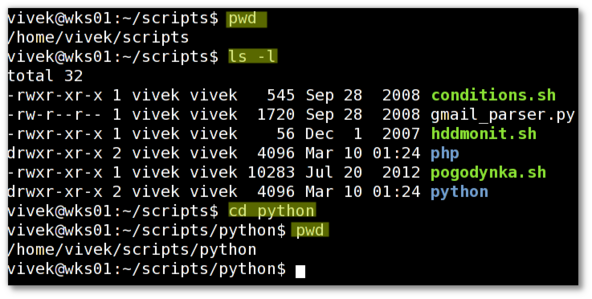
\includegraphics[width=0.5\textwidth]{figures/command.png}}
			\caption{Contoh command UNIX}
			\label{command}
			\end{figure}
		
		\subsection{Sejarah}
		\hspace*{1cm}UNIX adarah sistem operasi yang cepat dan kuat, karena dapat menampung banyak user sekaligus dan juga ideal untuk penyedialayanan internet.banyak ilmuan komputer yang berkata bahwa UNIX lebih baik dari windows karena lebih banyak fungsi dan dapat berkreasi di komputer lebih dalam. UNIX adalah sistem operasi yang paling banyak digunakan untuk server internet. UNIX dibuat pada tahun 1969, Versi awal dari UNIX file sistem terbuat dari hasil sketsa desain sebuah file sistem yang dikembangkan oleh Ken Thompson, Dennis Ritchie dan yang lainnya yang tergabung dalam General Electric Company and Project MAC of the Massachusetts Institute of Technology. Thompson dan Ritchie meng-implementasikan sistem mereka pada komputer PDP-7, termasuk versi awal UNIX file sistem, proses sub-sistem, dan beberapa set kecil dari utility programs, dan dan terlahirlah sistem baru yang dinamakan UNIX. Ritchie mengembangkan Bahasa Pemrograman B yang dihasilkan oleh Thompson menjadi satu yang dinamakan Bahasa Pemrograman C. lalu didistribusikan ke mahasiswa pada tahun 1970. Saat itu Amerika sedaang dalam perang dingin dan membutuhkan sistem komunikasi yang tahan dari ledakan nuklir. pada saat itu mreka masih menggunakan jaringan yang terpusat, jadi jika diserang dapat langsung tidak berfungsi. Mreka pun berfikir untuk menyambungkan setiap stasiun jaringan, jadi jika yang satu tidak berfungsi, masih ada yang lain. Pada saat itu mreka masih belum punya sistem operasi, mereka pun memilih UNIX dan jadilah Advanced Reseacrh Project Network atau yang kita kenal sebagai ARPANet.Setiap perusahaan besar pun punya UNIX versi mreka sendiri dikarenakan internet dijalankan oleh sistem operasi UNIX hal ini terjadi pada sekitar tahun 1978-1998. UNIX mendapatkan keuntungan karena merupakan pelopor pertama internet dan telah banyak digunakan. UNIX juga menunjukan beberapa efek dari jaringannya karena  seiring bertambahnya angka pengguna UNIX, bertambah pula program-program yang dibuat untuk para pengguna, dan banyak juga program yang dapat di unduh gratis. Para pengguna UNIX pun terus berkembang karena setiap ad bug, komunitas pengguna akan berusaha untuk membetulkannya. Lalu pasar sistem preasi pun mulai berbalik. Bill Gates membuat sistem operasinya sendiri yaitu DOS, lalu Apple pun mengeluarkan sistem operasi bikinannya sendiri yang menyatu dengan hardwarenya dan mempunyai graphic interface yang bagus. Lalu pasar mejadi lebih berbalik karena Bill Gates melisensi graphic interface nya Apple dan mengembangkan sistem operasi baru bernama windows. Sekarang, UNIX hanya dugunakan di tempat kerja saja. Walaupun UNIX adalah sistem operasi yang kuat, digunakan untuk banyak penelitian, membuat special effect untuk industri film, dan unggul dalam jaringan karena adalah sistem operasi yang digunakan untuk menjalankan internet juga untuk intranet, tetapi hal yang sangat krusial adalah banyak orang yang berfikir bahwa sistem operasi ini tidak user-friendly. Karena UNIX lebih fokus kepada fungsionalnya, tidak seperti Apple yang tefokus kepada grafis dan Microsoft yang terfokus kepada interaksi yang memudahkan pengguna. Disinilah kelemahan UNIX, mereka sudah tertinggal jauh sejak yang lain menggunakan graphic user interface dan sekarang kebanyak orang lebih memilih windows. walaupun UNIX dapat di unduh gratis tetapi hanya sedikit orang yang mau belajar dan menggunakannya, karena harus belajar sendiri tanpa di bimbing, dan juga sekarang tidak ada komputer atau laptop baru yang terinstall UNIX, karena mreka lebih memilih windows. Alasan utama lainnya adalah karna belum ada versi standard dari UNIX itu sendiri. Sebenarnya banyak versi UNIX dari sejak pengembangannya, tetapi sebenarnya ada dua versi utama, yang menyebabkan konflik para user. ATdanT adalah perusahaan pertama yang merilis UNIX untuk komunitas akademik tanpa menuntut biaya, tetapi saat UNIX mulai populer. pada tahun 1978, ATdanT mulai mengenakan biaya pada pengguna UNIX. Para mahasiswa Berkley menentang nya dan membuat versi mreka sendiri dan menamakannya BSD UNIX (Berkley Software Distribution). jadi UNIX mempunyai dua versi utama, yaitu versi ATdanT dan versi Sys V atau BSD. Kedua versi ini susah untuk dibedakan kecuali anda adalah programmer.
	
		\subsection{Versi}
		\begin{itemize}
			\item 1969 - UNIX pada PDP-7
			\item 1971 - UNIX Versi 1, pada DEC PDP-11/20
			\item 1973 - UNIX Versi 4, sudah menggunakan Bahasa Pemrograman C
			\item 1974 - UNIX Versi 5, untuk pendidikan
			\item 1975 - UNIX Versi 6, mulai timbul versi BSD
			\item 1979 - UNIX Versi 7, Portable dan dilengkapi kompiler dan Bourne Shell
			\item 1982 - UNIX System 3
			\item 1983 - UNIX System 5, ditambahkan versi BSD seperti vi dan c shell
			\item 1988 - UNIX System 5 Release 4, membuat semua program yang ditulis untuk System V dan Berkeley UNIX menjadi kompatibel dalam satu sistem.
		\end{itemize}
			\begin{figure}[ht]
			\centerline{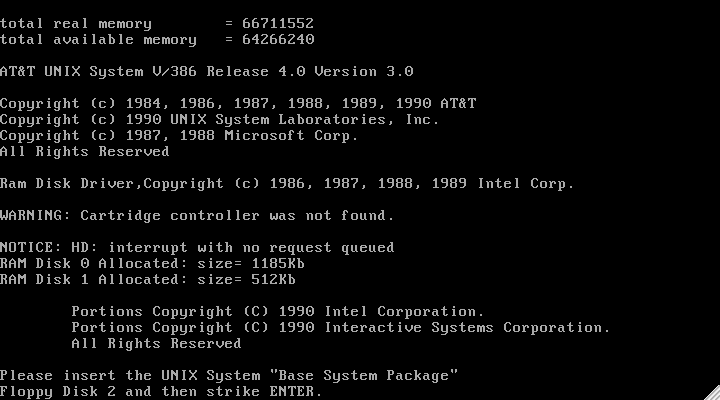
\includegraphics[width=1\textwidth]{figures/UNIXSVR4.png}}
			\caption{UNIX System V Release 4}
			\label{UNIXSVR4}
			\end{figure}
		Ini adalah contoh UNIX Versi 4 Release 4 \ref{UNIXSVR4}
		
		\subsection{Contoh}
		\begin{itemize}
			\item pwd : perintah ini artinya \"print working directory\" digunakan untuk mengetahui di direktori mana kita sedang berada.
			\item cd : perintah ini artinya \"change directory\" digunakan untuk berganti atau berpindah direktori.
			\item ls : perintah ini artinya \"list\" digunakan untuk melihat semua file dan folder dalam direktori dimana kita sedang berada.
			\item mkdir : perintah ini artinya \"make directory\" digunakan untuk membuat direktori atau folder baru.
			\item rmdir : perintah ini artinya \"remove directoy\" digunakan untuk menghapus direktori atau folder.
			\item clear : perintah ini digunakan untuk menghapus semua tampilan yang ada pada layar terminal.
			\item su : perintah ini digunakan untuk mengubah hak akses user menjadi root.
			\item ifconfig : perintah ini digunakan untuk melihat konfigurasi IP yang ada di network interface yang ada dalam PC kita.
			\item cp : perintah ini digunakan untuk membuat salinan dari sebuah file.
			\item mv : perintah ini digunakan untuk memindahkan suatu file dari direktori ke direktori lainnya.
		\end{itemize}
			\begin{figure}[ht]
			\centerline{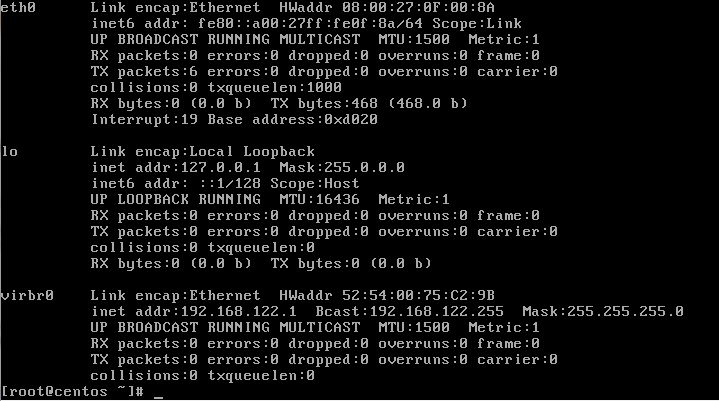
\includegraphics[width=1\textwidth]{figures/ifconfig.png}}
			\caption{Perintah untuk mengecek Network Interface}
			\label{ifconfig}
			\end{figure}
			
			\begin{figure}[ht]
			\centerline{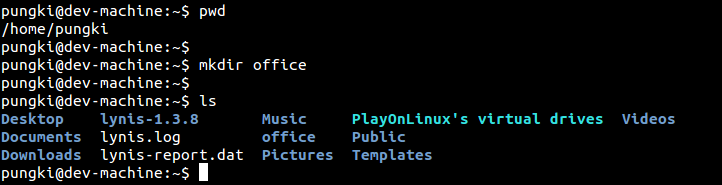
\includegraphics[width=1\textwidth]{figures/mkdir.png}}
			\caption{Perintah untuk membuat folder}
			\label{mkdir}
			\end{figure}
		Dibawah ini adalah contoh perintah ifconfig \ref{ifconfig}
		Dibawah ini adalah contoh perintah mkdir \ref{mkdir}
		
\pagebreak
	
	\section{Perintah Pada DOS}
		\subsection{Definisi}
		\hspace{1cm}Perintah pada DOS merupakan perintah atau command yang dapat dijalankan pada sistem operasi DOS. terdapat 2 jenis perintah dalam DOS, yaitu perintah internal, yaitu perintah yang sudah ada dalam COMMAND.COM (interpreter perintah DOS), dapat langsung di eksekusi oleh kernel DOS, seperti: Date, Time, Copy, atau juga Del. sedangkan perintah eksternal, yaitu perintah yg tidak ada dalam COMMAND.COM, dan memerlukan sebuah file yang dapat dieksekusi dan terdapat didalam direktori aktif, Seperti: fdisk, format, ataupun edit.
		
		\vspace{1cm} Ini adalah contoh perintah - perintah yang dilakukan pada DOS 
		\ref{commanddos}
		\begin{figure}[ht]
			\centerline{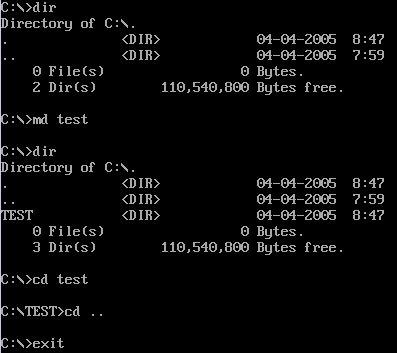
\includegraphics[width=0.5\textwidth]{figures/commanddos.png}}
			\caption{Perintah Pada DOS}
			\label{commanddos}
			\end{figure}
			
		\subsection{Sejarah}
		\hspace{1cm}Pada pertengahan tahun 1980, Tim Paterson membuat sistem operasi yang dinamakan 86-DOS, yang merupakan cikal bakal MS-DOS. Pada tahun 1981, Microsoft membeli hak cipta 86-DOS, membuat perubahan besar, dan mengubah namanya menjadi MS-DOS. MS-DOS pertama kali digunakan pada PC-DOS 1.0 yang dikeluarkan pertama kali oleh IBM dan menjadi PC pertama yang dibuat oleh IBM pada musim gugur tahun 1981. Pada tahun 1982 bulan juni IBM merilis MS-DOS 1.25 untuk memperbaiki beberapa bug dan agar bisa mendukung double-sided disks dan meningkatkan independesi hardware di kernel DOS. Versi ini dikeluarkan jg oleh beberapa vendor selain IBM, seperti COMPAQ, Columbia, dan yang lainnya, MS-DOS versi 1.0 pun tidak lagi digunakan. MS-DOS versi 2.0 pun dirilis pada bulan maret tahun 1983, dan mengalami banyak peningkatan dari versi sebelumnya, seperti mendukung disket yang memiliki kapasitas besar, mendukung penggunaan shell, dan yang lainnya. tidak lama kemudia keluar MS-DOS 2.11 untuk meningkatkan kualitas penggunaan seperti 16-bit huruf kanji, dan beberapa bugs. MS-DOS versi 2.25, rilis pada bulan oktober tahun 1985 yang di distribusi ke bagian timur dan tidak pernah rilis di eropa dan United States. MS-DOS 3.0 di keluarkan oleh IBM pada bulan agustus tahun 1984 yang menambahkan fitur baru seperti penambahan format mata uang dunia, meluaskan pelaporan error dan yang lainnya. MS-DOS versi 4 pun di rilis pada tahun 1988 dengan meningkatkan visual shell dan mendukung file sistem yang lebih besar. Selama MS-DOS mengalami peningkatan, Microsoft dengan berusaha membuat sistem operasi yang menggunakan user interface dan multitasking, dan terlahirlah Microsoft Windows.
		\vspace{1cm} Ini adalah contoh MS-DOS Versi 3.0 \ref{win31}
		\begin{figure}[ht]
			\centerline{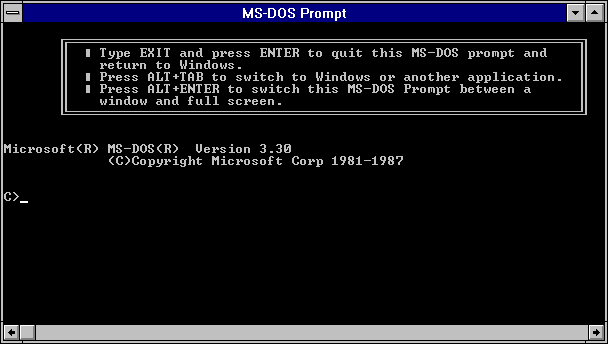
\includegraphics[width=0.5\textwidth]{figures/win31.png}}
			\caption{MS-DOS Versi 3.0}
			\label{win31}
			\end{figure}
		
		\subsection{Versi}
		\begin{itemize}
			\item MS-DOS 1.0 - 1981, Sistem operasi pertama pada IBM PC
			\item MS-DOS 1.1 - Lebih banyak di distribusikan oleh OEMS dibandingkan IBM
			\item MS-DOS 1.25 - Perbaikan beberapa bugs
			\item MS-DOS 2.0 - Struktur file dan ditambahkan hard-disk
			\item MS-DOS 2.01 - Dikenalkan dengan PCjr
			\item MS-DOS 2.11 - Perbaikan beberapa bug di MS-DOS Versi 2.01
			\item MS-DOS 3.0 - ditambahkan hard disk yang lebih besar
			\item MS-DOS 3.1 - Mendukung Jaringan Microsoft
			\item MS-DOS 3.2 - Mendukung disk ukuran 3.5 inch
			\item MS-DOS 4.0 - Mendukung logical volume lebih besar dari 32 MB, visual shell
		\end {itemize}
		
		\vspace{1cm} Ini adalah contoh MS-DOS Versi 4.0 \ref{dosv4}
		\begin{figure}[ht]
			\centerline{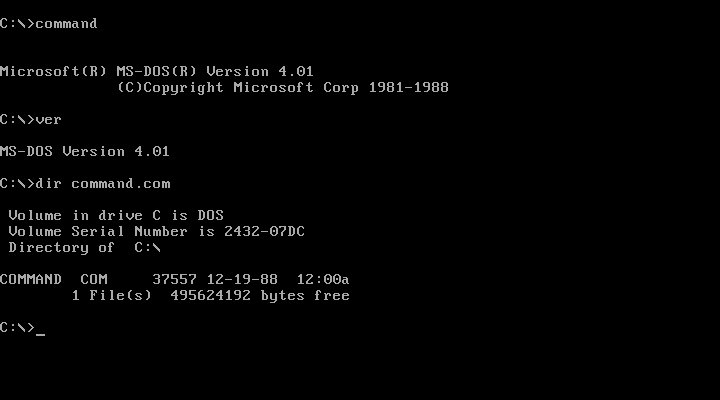
\includegraphics[width=0.5\textwidth]{figures/dosv4.png}}
			\caption{MS-DOS Versi 4.0}
			\label{dosv4}
			\end{figure}
		
		\subsection{Contoh}
		\begin{itemize}
			\item Chdir / CD : yang artinya \"change directory\" untuk berpindah direktori
			\item CLS : yang artinya \"clear screen\" untuk menghapus atau mengosongkan semua teks yang ada di layar
			\item Del : yang artinya \"delete\" untuk menghapus file atau beberapa file yang dinyatakan
			\item Mkdir / MD : yang artinya \"make directory\" untuk membuat suatu direktori atau folder
			\item Prompt : digunakan untuk mengubha prompt yang di gunakan di MS-DOS
			\item Time : digunakan untuk menampilkan atau mengatur jam pada sistem
			\item CD.. : digunakan untuk kemabali 1 level direktori di atasnya
			\item Vol : yang artinya \"volume\" untuk menampilkan label pada drive tertentu dan serial numbernya
			\item Ver : yang artinya \"versi\" untuk menampilkan versi dari dos yang dipakai
			\item Tree : untuk menampilkan direktori dengan semua direktori yang terdapat didalamnya dengan bentuh diagram (pohon)
			\item Deltree : untuk menghapus direktori beserta seluruh isinya
		\end{itemize}
		Ini adalah contoh perintah date pada DOS \ref{date}
		Ini adalah contoh perintah dir pada DOS \ref{dir}
			\begin{figure}[ht]
			\centerline{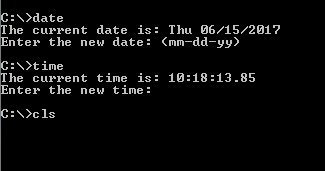
\includegraphics[width=0.5\textwidth]{figures/date.png}}
			\caption{Perintah untuk melihat dan mengatur jam dan tanggal}
			\label{date}
			\end{figure}
			
			\begin{figure}[ht]
			\centerline{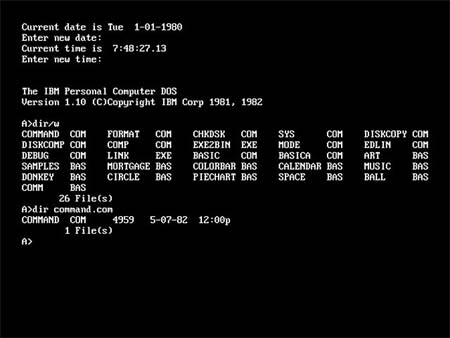
\includegraphics[width=0.5\textwidth]{figures/dir.jpg}}
			\caption{Perintah untuk melihat daftar file di direktoris}
			\label{dir}
			\end{figure}
			
\newpage

	\vspace*{1,5cm}Artikel yang dirangkum dari sebuah buku yang berjudul The design of the UNIX operating system \cite{bach1986design}.
		
	\vspace*{1cm}Artikel The UNIX System: The Evolution of the UNIX TIme-sharing System \cite{ritchie1984unix}.
	
	\vspace*{1cm}Artikel yang dirangkum dari sebuah buku yang berjudul UNIX: Teknik Penguasaan Secara Sistematis \cite{setiawanunix}
	
	\vspace*{1cm}Artikelyang dirangkum dari sebuah buku yang berjudul Advanced MS-DOS Programming \cite{duncan1988advanced}.